%%%%%%%%%%%%%%%%%%%%%%%%%%%%%%%%%%%%%%%%%%%%%%%%%%%%%%%%%%%%%%%%%%%%%%%%%%%%%%%%
%%% Results
%%%%%%%%%%%%%%%%%%%%%%%%%%%%%%%%%%%%%%%%%%%%%%%%%%%%%%%%%%%%%%%%%%%%%%%%%%%%%%%%

\clearpage
\section{Discussion}
\label{sec:discussion}

In this section I will describe the results of my research and development.
I will describe the final product developed in this project and list the numerical data from the machine learning experiments.
Lastly, I will evaluate the results of this thesis based on the initial research questions.

\subsection{Results}

%T\"ass\"a osassa esitet\"a\"an tulokset ja vastataan tutkielman alussa
%esitettyihin tutkimuskysymyksiin. Tieteellisen kirjoitelman
%arvo mitataan t\"ass\"a osassa esitettyjen tulosten perusteella.

\begin{figure}[htb]
\centering 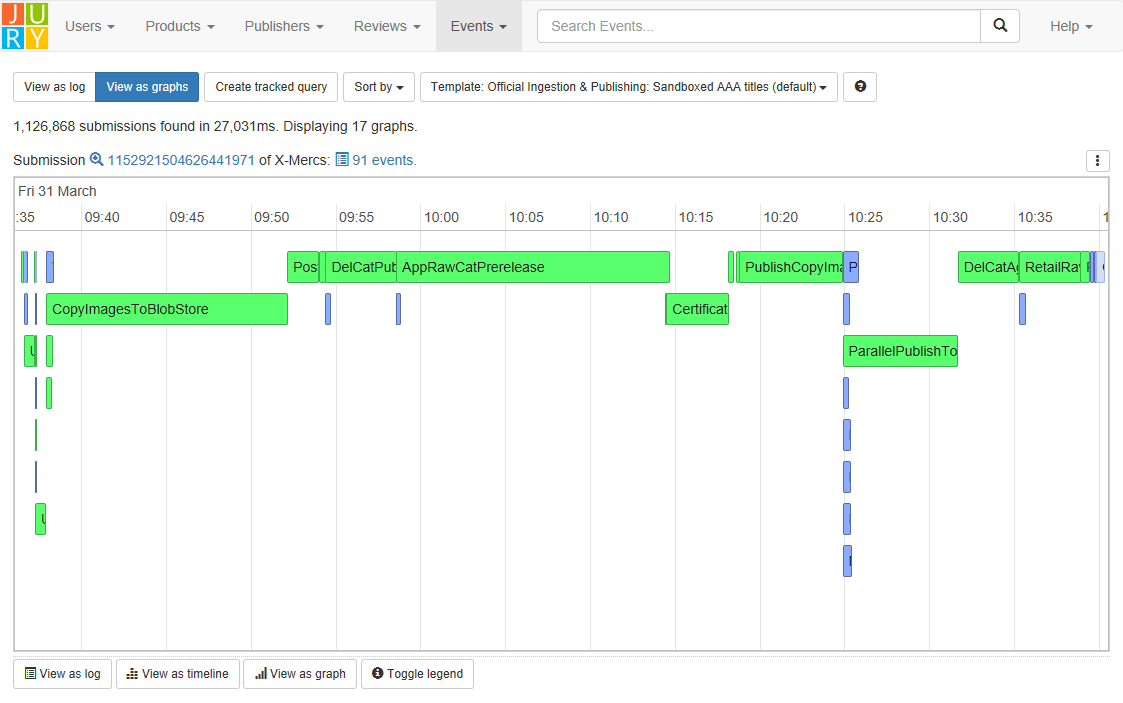
\includegraphics[width=\linewidth]{gfx/screenshots/timeline.png}
\caption{Timeline view \label{fig:timeline}}
\end{figure}

\begin{figure}[htb]
\centering 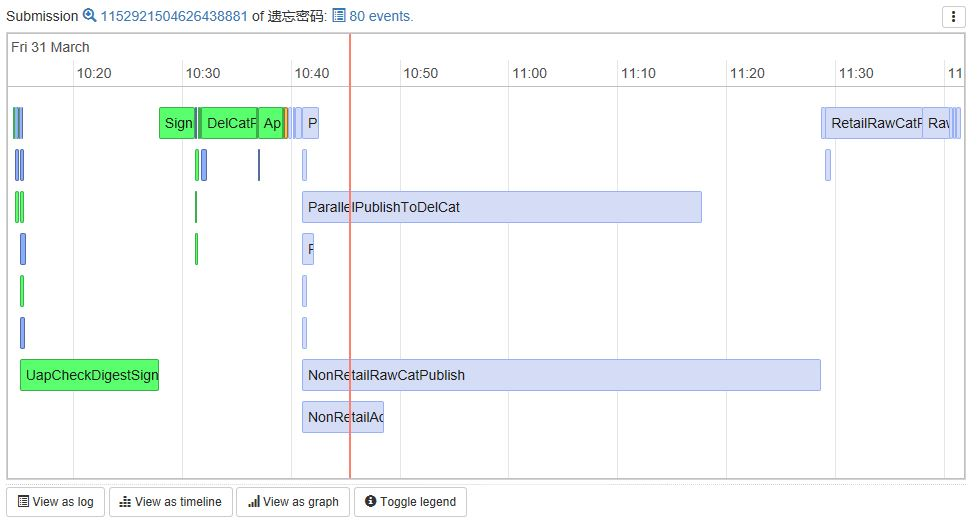
\includegraphics[width=\linewidth]{gfx/screenshots/estimates.jpg}
\caption{Timeline view with estimates \label{fig:estimates}}
\end{figure}

\begin{figure}[htb]
\centering 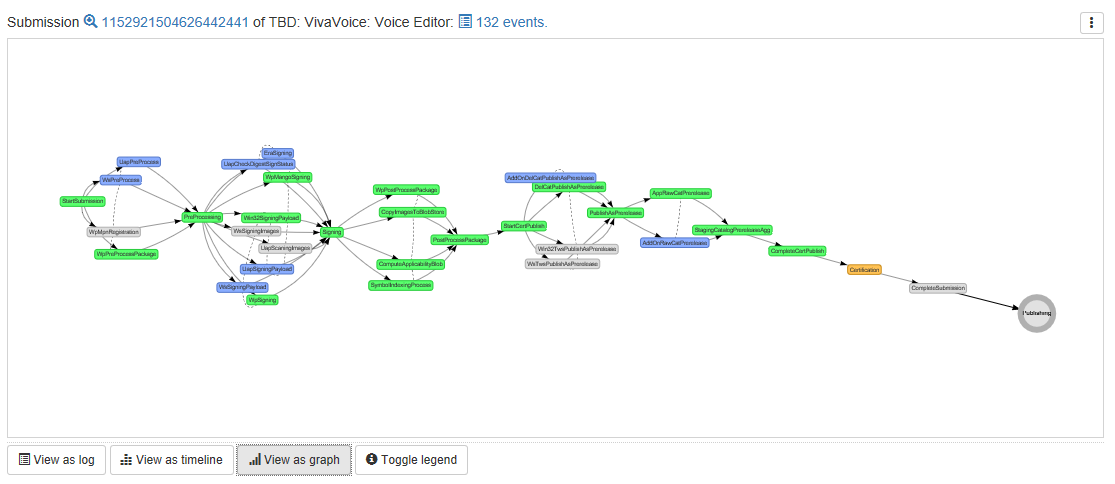
\includegraphics[width=\linewidth]{gfx/screenshots/graph.png}
\caption{Graph view \label{fig:graph}}
\end{figure}

Figure \ref{fig:timeline} shows the final product developed in this thesis.
The topmost bar is the main navigation of the website in which the user can write a query to search for events.
The page below can display any number of traces corresponding to the events that match the user's query.
If a large number of traces would be returned, the view is paged.
The second bar under the navigation is the event navigation bar I developed, which includes all the functionality that affects all the content on the event-related pages.
It allows the user to switch between the log view (See figure \ref{fig:plaineventlog}) and the visualizations.
It also includes functionality for sorting the visualizations and choosing which process model to build the visualization from.

Each trace returned by the query is visualized as a timeline or a graph. On top of the visualization the user can see the basic information about the trace containing the submission ID and the name of the product.
Under the visualization there are options to choose how the visualization is displayed (between the log view, the graph view, and the timeline view) and an option to toggle help.
The visualization can be manipulated with the mouse or a touch screen. It allows panning and zooming actions.
The user can select or mouseover individual events to see all the metadata related to the event.

In the timeline view (figure \ref{fig:timeline}) the visualization is set on top of a horizontal axis that corresponds to time. The activities shown have start and end times which can be seen visually or in the metadata.
Parallel activities are stacked on top of each other.
Figure \ref{fig:estimates} shows the estimations for an incomplete submission.
The activities yet to happen are drawn with a faint blue color and their estimated start and end times are visualized similarly as the logged activities.
The red line displays the current time.
The user can visually see the status of the submission and the activities that are predicted to have happened already.

Figure \ref{fig:graph} shows the alternate directed graph view. In the graph view the directed graph is drawn for the user. The graph nodes are interactive and the edges act as two-dimensional springs.
The user can thus manipulate and move the nodes. Panning and zooming actions are also enabled.

In the user meetings in between the two iterations the timeline view was unanimously agreed to be the more useful visualization. 
The graph view was seen as ``unnecessarily complex'' and the physics animation was perceived as ``annoying'' and ``fidgety''. 
In other words, the graph view didn't offer a clear ``big picture'' since it required the user to manipulate the view before it showed the information clearly. 
The users wanted the graph view to have more organization, and several users asked for automated sorting or positioning of the graph nodes.

Conversely, the static and clear positioning of the timeline view was seen as useful.
Since the view was pre-generated and organized on a static timeline, most graphs would end up looking exactly the same without any manipulation.
A user would be able to visually scan the list of graphs and notice anything significantly different.
The user could then investigate the distinct graph to find out whether the difference is a result of a failure.
The users commented that they did not even need to pay attention to the specific nodes but only focus on the overall shape of the graph.

To evaluate the results of the machine learning models, I first calculated a baseline for comparison.
The baseline consists of the same simple statistics as were used for the estimates in the application, the TP50 (median) and the TP75.
I calculated these two values for each transition (graph edge) based on the training set to construct a simple model. 
In the model each transition corresponds to a single value (the TP50 or the TP75). 
When predicting, the model always returns this value based on the transition in question.
Table \ref{tab:statresults} lists the results from this baseline model for both training datasets described in section \ref{sec:ml-estimation}. 
The values of \textit{mean absolute error} and \textit{root mean square error} are listed.
\nyi{should I explain what these are?}

\begin{table}[htb]
\begin{center}
\begin{tabularx}{\linewidth}{| X | r | r |}
\hline
Dataset + Model & Mean Absolute Error & RMSE \\
\hline
\textbf{JSON template} &  & \\
TP50 value (median)         & 573.3 & 5871.4 \\
TP75 value                  & 710.5 & 5484.2 \\
\hline
\textbf{Automatically generated template} &  & \\
TP50 value (median)         & 919.6 & 9937.3 \\
TP75 value                  & 954.0 & 9904.8 \\
\hline
\end{tabularx}
\end{center}
\caption{Results from plain statistics}
\label{tab:statresults}
\end{table}

I used the same training and testing sets to find the same error values for each machine learning model.
The error values are listed in table \ref{tab:mlresults}.
The first two columns list the error values for the boosted decision trees model (BDT).
Again, the values of mean absolute error (``Absolute'') and root mean square error (``RMSE'') are listed.
The same models are used for both datasets.

I calculated the error values for all the different sets of features, as described in section \ref{sec:featureset}
.
The first model was generated by only using the features available in the application package.
The second model uses the current time in seconds since the submission start as an additional feature.
The next two models use the new features I created for resubmissions and entering a manual review.
I also used both these two features together to test the models, and lastly all these three features combined.

\begin{table}[htb]
\begin{center}
\begin{tabularx}{\linewidth}{| X | r | r | r | r |}
\hline
~ & \multicolumn{2}{c|}{BDT} & \multicolumn{2}{c|}{Poisson} \\
Dataset + Model & Absolute & RMSE & Absolute & RMSE \\
\hline
\textbf{JSON template} &  &  &  &  \\
No extra features                   & 809.1 & 6290.7 & 881.1 & 5970.6 \\
with current time                   & 825.2 & 6130.3 & 881.1 & 5971.0 \\
with manual review                  & 689.7 & 5819.0 & 809.3 & 5800.9 \\
with resubmission                   & 831.5 & 6255.3 & 881.1 & 5971.2 \\
with manual review and resubmission & 703.7 & 5807.5 & 808.9 & 5800.8 \\
with all extra features             & 693.5 & 5801.9 & 808.3 & 5800.4 \\
\hline
\textbf{Automatically generated template} &  &  &  &  \\
No extra features                   & 994.8 & 5756.3 & 1243.9 & 6563.3 \\
with current time                   & 1099.7 & 6470.5 & 1225.8 & 6558.7 \\
with manual review                  & 815.1 & 5332.1 & 1038.5 & 5785.0 \\
with resubmission                   & 1004.3 & 5845.3 & 1219.1 & 6553.8 \\
with manual review and resubmission & 806.5 & 5428.4 & 1038.4 & 5785.7 \\
with all extra features             & 787.8 & 5234.4 & 1038.6 & 5785.4 \\
\hline
\end{tabularx}
\end{center}
\caption{Results from the best ML models}
\label{tab:mlresults}
\end{table}

\subsection{Evaluation}
\label{sec:evaluation}

% % Tutkimustuloksien merkityst\"a on aina syyt\"a arvioida ja tarkastella
% % kriittisesti.  Joskus tarkastelu voi olla t\"ass\"a osassa, mutta se
% % voidaan my\"os j\"att\"a\"a viimeiseen osaan, jolloin viimeisen osan nimeksi
% % tulee >>Tarkastelu>>. Tutkimustulosten merkityst\"a voi arvioida my\"os
% % >>Johtop\"a\"at\"okset>>-otsikon alla viimeisess\"a osassa. 

% % T\"ass\"a osassa on syyt\"a my\"os arvioida tutkimustulosten luotettavuutta.
% % Jos tutkimustulosten merkityst\"a arvioidaan >>Tarkastelu>>-osassa,
% % voi luotettavuuden arviointi olla my\"os siell\"a. 

%\item How can a real-time event log from multiple sources and multiple concurrent workflows be dynamically transformed into a model that describes the process? 
%\nyi{Talk about success with graph generation}\\

The goal of this thesis was to find out whether past event logs could be used to detect anomalies in real-time. 
The first research question asked how event log data can be used to generate a model that describes the process.
In this thesis I explored the options of using WF-nets and directed graphs to model processes.
The directed graphs were chosen to be satisfactory for modeling the workflows in the Microsoft Store.
The models were visualized as both directed graphs and on a horizontal timeline.
The users found the static and pre-arranged timeline view to be useful. 
However, the graph view was deemed to be useful for debugging the process, since it shows the relationships and dependencies between the activities.
For this reason I kept both views as options for the user to choose from.

%\nyi{Finding bugs in system (race conditions!) based on graphs}\\
The models were evaluated by comparing them to the official workflow descriptions that were used by engineers to maintain the models. 
With a short time span of events the models were noisy and lacked some of the parallelism that the real processes had.
However, with event logs longer than three days the models captured all the activities and their dependencies.
In one instance the graph showed incorrect dependencies which proved to be a race condition bug in the actual system that caused the process workflow to execute in an invalid order.
The results from the discovered model were used to fix the race condition in the store system.

%\nyi{Changes in the system reflected real time (also a strength?)}\\
The model was always generated from the past three days or seven days of data, based on the query. Because of this, any changes to the workflows started to appear in the models within this time window. 
The changes were automatically picked up by the process discovery algorithm and required no engineer interaction.

%\item How can the model and past log data be used to predict future events and their times?
The second research question asked how the model could be used to predict future events and their times. 
The predictions I ended up using in the thesis were based on simple statistics. 
The statistical approach was deemed to be sufficient for the use case of predicting activities. 
Since many of the activities are fairly short, small variations in the predictions are acceptable. 
In addition, an overestimation is always a better result in this use case.
For example, if an event is estimated to arrive in five minutes and it arrives in four, the user is happy.
Since the system has a lot of variation in activity durations even when the system is functioning normally, detecting small anomalies is not useful to the user and can even be seen as noise.

Machine learning was considered an option to improve the predictions. The idea was that the variation in delay would depend on the characteristics of the submission such as the file size.
However, the machine learning models did not significantly improve the results of the predictions.
When comparing the results for the simple statistical model using the median and the TP75 values (figure \ref{tab:statresults}) and the results from the machine learning models (figure \ref{tab:mlresults}) there is no significant difference.
With the first data set (``JSON template'') the machine learning models did not even reach the error values of the statistical approach.
With the second data set (``Automatically generated template'') the machine learning model showed a slight improvement over the statistical model.
However, since most of the activities have lengths of less than five minutes, an average prediction error of more than 10 minutes is still not a good prediction.
Since slightly overestimating an ETA was seen as acceptable by the users, the complexity and engineering work required to implement the machine learning models in production was not seen as necessary.
A simple statistical implementation with simpler code was seen as more worthwhile than a possible slight increase in prediction accuracy.

%\nyi{Talk about negatives with machine learning models}\\
%\nyi{Reason why they didn't end up working}

The reasons why the machine learning models did not provide useful results can be explored.
Since both models (Poisson regression and boosted decision trees) reached similar results even though they function very differently, it suggests that the data sets were too noisy or the results did not depend enough on the used features.
Even after I identified the two possible features that could be added to the data sets (the manual review feature and the resubmission feature), it did not significantly improve the results.
The result from my exploration was that other features such as time of day, system congestion and network status was affecting the times more than the characteristics of the application package itself.

In conclusion, the users agreed that the statistical estimations were useful in the visualizations, since they allow the user to visually see what part of the workflow the submission is in.
Furthermore, the predictions give the user a simple estimate for the completion time. 
For many users, the exact time is not important, but knowing whether the estimation is in the order of minutes or hours was seen as significant.

%\item How can the predictions be used to detect anomalies in new events (or lack thereof)?

The third and final research question asked if the predictions could be used to automatically notify the users about anomalies without the need for the user to look at the visualizations.
The main use case was to detect submissions that are ``stuck''.
The expression ``stuck'' meant a submission that has stayed in a particular activity for an abnormally long period of time, usually because of an error in the submission data or in the activity processor.
This means that the system should send a notification to a relevant user about any significant anomalies, whereas small anomalies are not important.
The notification system described in section \ref{sec:notifications} was proven to function correctly after the initial testing. 
However, since the number of stuck submissions is very small compared to the massive amount of submissions in the store, accurate evaluation was difficult to make during my short evaluation period.

The project was released into the production systems and has been in use in Jury.
At the time of this writing (July 2017) in the past 90 days 232 unique users have used the events-section of Jury, and of those users 157 have used the workflow visualizations.
Only seven users currently use the automatic email notification features.

%%%%%%%%%%%%%%%%%%%%%%%%%%%%%%%%%%%%%%%%%%%%%%%%%%%%%%%%%%%%%%%%%%%%%%%%%%%%%%%%

\subsection{Conclusions} 
\label{sec:conclusions}

This thesis research achieved its main goal, which was to create visualizations for the internal Microsoft users to help maintain and monitor the store systems and submissions.
The system was released into production immediately and all the users using Jury are now able to use the events, visualizations, and the notification system.

More than 150 users have used the notifications within the past three months which I consider significant, 
since the users of Jury are all internal and most of them are users from a few specific teams within the company.
The notification system needs to be publicized within the company more, since it seems that most users are not aware it exists.

The accuracy of the models and the real-time overlay functionality was praised by the users and is seen as a success.
Most studies I referenced in this thesis focus on analyzing past logs to find useful information.
My thesis work had a significant focus on the real-time functionality and the ability to dynamically adapt to the events as they arrive.
I was able to successfully use the events and leverage the process models in a real-time scenario.

\subsubsection{Limitations and Future work}

Further research should be made into the process discovery algorithm options.
This study only focused on the \textalpha-algorithm and its applications. 
Different graph generation algorithms such as transition systems \cite{van2013discovering} should be explored and tested in this particular application.

The current system's prediction accuracy is acceptable but not particularly accurate.
For accurate predictions and better machine learning possibilities more research is needed on the aspects of the store which affect the activity processing times.

Furthermore, the real-time aspect of process mining is something that needs further examination. In this thesis I adapted existing methods designed for analyzing past event logs to be used in a real-time scenario.
Further research should be made to specifically examine the challenges and possibilities of real-time events.

